\documentclass[twoside]{article}
\setlength{\oddsidemargin}{-0.5 in}
\setlength{\evensidemargin}{1.5 in}
\setlength{\topmargin}{-0.6 in}
\setlength{\textwidth}{5.5 in}
\setlength{\textheight}{8.5 in}
\setlength{\headsep}{0.5 in}
\setlength{\parindent}{0 in}
\setlength{\parskip}{0.07 in}
\setlength{\marginparwidth}{145pt}

%
% ADD PACKAGES here:
% 12

\usepackage{amsmath,
            amsfonts,
            amssymb,
            graphicx,
            mathtools,
            flexisym,
            marginnote,
            hyperref,
            titlesec}

\usepackage[english]{babel}
\usepackage[utf8]{inputenc}
\usepackage[shortlabels]{enumitem}

\graphicspath{ {images/} }

\hypersetup{
    colorlinks=true,
    linkcolor=blue,
    filecolor=magenta,      
    urlcolor=blue,
}

\titlespacing\section{0pt}{12pt plus 4pt minus 2pt}{0pt plus 2pt minus 2pt}
\titlespacing\subsection{0pt}{12pt plus 4pt minus 2pt}{0pt plus 2pt minus 2pt}

%
% The following commands set up the lecnum (lecture number)
% counter and make various numbering schemes work relative
% to the lecture number.
%
\newcounter{lecnum}
\renewcommand{\thepage}{\thelecnum-\arabic{page}}
\renewcommand{\thesection}{\thelecnum.\arabic{section}}
\renewcommand{\theequation}{\thelecnum.\arabic{equation}}
\renewcommand{\thefigure}{\thelecnum.\arabic{figure}}
\renewcommand{\thetable}{\thelecnum.\arabic{table}}

\newcommand{\aosv}{1044414: Advanced Operating Systems and Virtualization}
\newcommand{\wir}{1038137: Web Information Retrieval}
\newcommand{\va}{1052057: Visual Analytics}
\newcommand{\advprog}{1044416: Advanced Programming}
\newcommand{\dchpc}{1044399: Data Centers and High Perf. Computing}

\newcommand{\qu}[1]{\marginnote{\textcolor{cyan}{#1}}}


%
% The following macro is used to generate the header.
%
\newcommand{\lecture}[4]{
   \pagestyle{myheadings}
   \thispagestyle{plain}
   \newpage
   \setcounter{lecnum}{#4}
   \setcounter{page}{1}
   \noindent
   \begin{center}
   \framebox{
      \vbox{\vspace{2mm}
    \hbox to 7.4in { {\bf #1
    \hfill Spring 2018} }
       \vspace{4mm}
       \hbox to 7.4in { {\Large \hfill Lecture #4: #2  \hfill} }
       \vspace{2mm}
       \hbox to 7.4in { {\it Lecturer: #3 \hfill Scribe: Anxhelo Xhebraj} }
      \vspace{2mm}}
   }
   \end{center}
   \markboth{Lecture #4: #2}{Lecture #4: #2}

   \iffalse
   {\bf Note}: {\it LaTeX template courtesy of UC Berkeley EECS dept.}

   {\bf Disclaimer}: {\it These notes have not been subjected to the
   usual scrutiny reserved for formal publications.  They may be distributed
   outside this class only with the permission of the Instructor.}
   \vspace*{4mm}
   \fi
}
%
% Convention for citations is authors' initials followed by the year.
% For example, to cite a paper by Leighton and Maggs you would type
% \cite{LM89}, and to cite a paper by Strassen you would type \cite{S69}.
% (To avoid bibliography problems, for now we redefine the \cite command.)
% Also commands that create a suitable format for the reference list.
\iffalse
\renewcommand{\cite}[1]{[#1]}
\def\beginrefs{\begin{list}%
        {[\arabic{equation}]}{\usecounter{equation}
         \setlength{\leftmargin}{2.0truecm}\setlength{\labelsep}{0.4truecm}%
         \setlength{\labelwidth}{1.6truecm}}}
\def\endrefs{\end{list}}
\def\bibentry#1{\item[\hbox{[#1]}]}
\fi

%Use this command for a figure; it puts a figure in wherever you want it.
%usage: \fig{NUMBER}{SPACE-IN-INCHES}{CAPTION}
\newcommand{\fig}[3]{
            \vspace{#2}
            \begin{center}
            Figure \thelecnum.#1:~#3
            \end{center}
    }
% Use these for theorems, lemmas, proofs, etc.
\newtheorem{theorem}{Theorem}[lecnum]
\newtheorem{lemma}[theorem]{Lemma}
\newtheorem{proposition}[theorem]{Proposition}
\newtheorem{claim}[theorem]{Claim}
\newtheorem{corollary}[theorem]{Corollary}
\newtheorem{definition}[theorem]{Definition}
\newenvironment{proof}{{\bf Proof:}}{\hfill\rule{2mm}{2mm}}

% **** IF YOU WANT TO DEFINE ADDITIONAL MACROS FOR YOURSELF, PUT THEM HERE:

\newcommand\E{\mathbb{E}}

\begin{document}

\nocite{*}

%FILL IN THE RIGHT INFO.
%\lecture{**LECTURE-NUMBER**}{**DATE**}{**LECTURER**}{**SCRIBE**}

\lecture{\aosv}{March 16}{Alessandro Pellegrini}{5}

%\footnotetext{These notes are partially based on those of Nigel Mansell.}

% **** YOUR NOTES GO HERE:

In this lecture we will look into the organization and initialization of memory of the linux i386 kernel v. = 2.4.22.

\section{Early Paging}

As we anticipated in Lecture 3 (Sec 3.4) paging is enabled in \texttt{startup_32} through the following instructions \marginnote{\texttt{ENTRY(swapper_pg_dir) \\
    .long 0x00102007 // pg0 \\
    .long 0x00103007 // pg1 \\
    .fill BOOT_USER_PGD_PTRS-2,4,0 \\
    /* default: 766 entries */ \\
    .long 0x00102007 \\
    .long 0x00103007 \\
    /* default: 254 entries */ \\
    .fill BOOT_KERNEL_PGD_PTRS-2,4,0}}[1cm]

\begin{verbatim}
> arch/i386/kernel/head.S
    movl $swapper_pg_dir-__PAGE_OFFSET, %eax
    movl %eax, %cr3
    movl %cr0, %eax
    orl $0x80000000, %eax
    movl %eax, %cr0
\end{verbatim}

where \texttt{swapper_pg_dir} is a label corresponding to the virtual address of the first level page table and \texttt{__PAGE_OFFSET} is \texttt{0xc0000000} (3GB, which is the virtual address of the kernel in i386). \texttt{\%cr3} is not directly set to \texttt{swapper_pg_dir}, but the value shown above which is the physical address of \texttt{swapper_pg_dir} (the difference between virtual and physical addresses of the kernel is just an offset). In \texttt{startup_32} the kernel initializes its page tables
to span only the first 8MB of the kernel. This is done by initializing two Page Tables (last level) found at label \texttt{pg0} and creating 4 entries in the first level page table (pointed by \texttt{swapper_pg_dir}): entry 0 and \texttt{0x300} (768) contain in the address field the physical address of \texttt{pg0} while entry 1 and \texttt{0x301} (769) contain the
physical address of \texttt{pg1}. When paging is enabled, given the configuration of the page table we have that both the virtual addresses \texttt{0x0} to \texttt{0x007fffff} (from 0 to 8MB) and \texttt{0xc0000000} to \texttt{0xc07fffff} (from 3GB to 3GB + 8MB) will map to the physical addresses \texttt{0x0} to \texttt{0x007fffff}. The former is called \textit{identity map} since maps the first 8MB of virtual addresses to the first 8MB of physical addresses while the latter is
called \textit{kernel map} since it maps the virtual addresses of the kernel to its physical addresses.

\section{Bootmem Allocator}

The transition from 8MB to 896MB of virutal memory is performed in the \texttt{start_kernel()} function in \texttt{init/main.c}. This function calls \texttt{setup_arch()} defined in \\ 
\texttt{arch/i386/kernel/setup.c} (architecture dependent code) which initializes various data structures with among them the Bootmem allocator. The Bootmem allocator is a data structure and a set of functions that is used by the kernel to allocate memory (at the granularity of page sizes, 4KB) before the kernel Main Memory subsytem is setup. This set of APIs is available only at early setup of memory therefore it has \texttt{__init} in its signature.

The bootmem allocator initialization is performed in \texttt{setup_memory()}
implemented in \texttt{arch/i386/kernel/setup.c} through the
\texttt{init_bootmem()} function (\texttt{mm/bootmem.c}) initializing a bitmap
where each bit
refers to a page frame in the range of physical addresses \texttt{_end}
(after the last section of the decompressed kernel image) up to 896MB.
First all the bits are set to 1 meaning that no page can be used for
allocation. After that it is up to the function
\texttt{register_bootmem_low_pages()} to query the E820 table and set the bits
of free page frames to 0.

\iffalse
\section{Kenel-Level MM Data Structures}

\begin{itemize}
    \itemsep-2pt
    \item First is a memory mapping for kernel code and data. 
    \item Core map: set of data structures to keep information about every frame of physical memory. (NUMA, different cores see only a subportion of ram) If a region is not available to a core then it has to the "owner" core for that address.
    \item Free list of physical memory frames
\end{itemize}
\fi

\section{Paging in Linux}

\begin{center}
  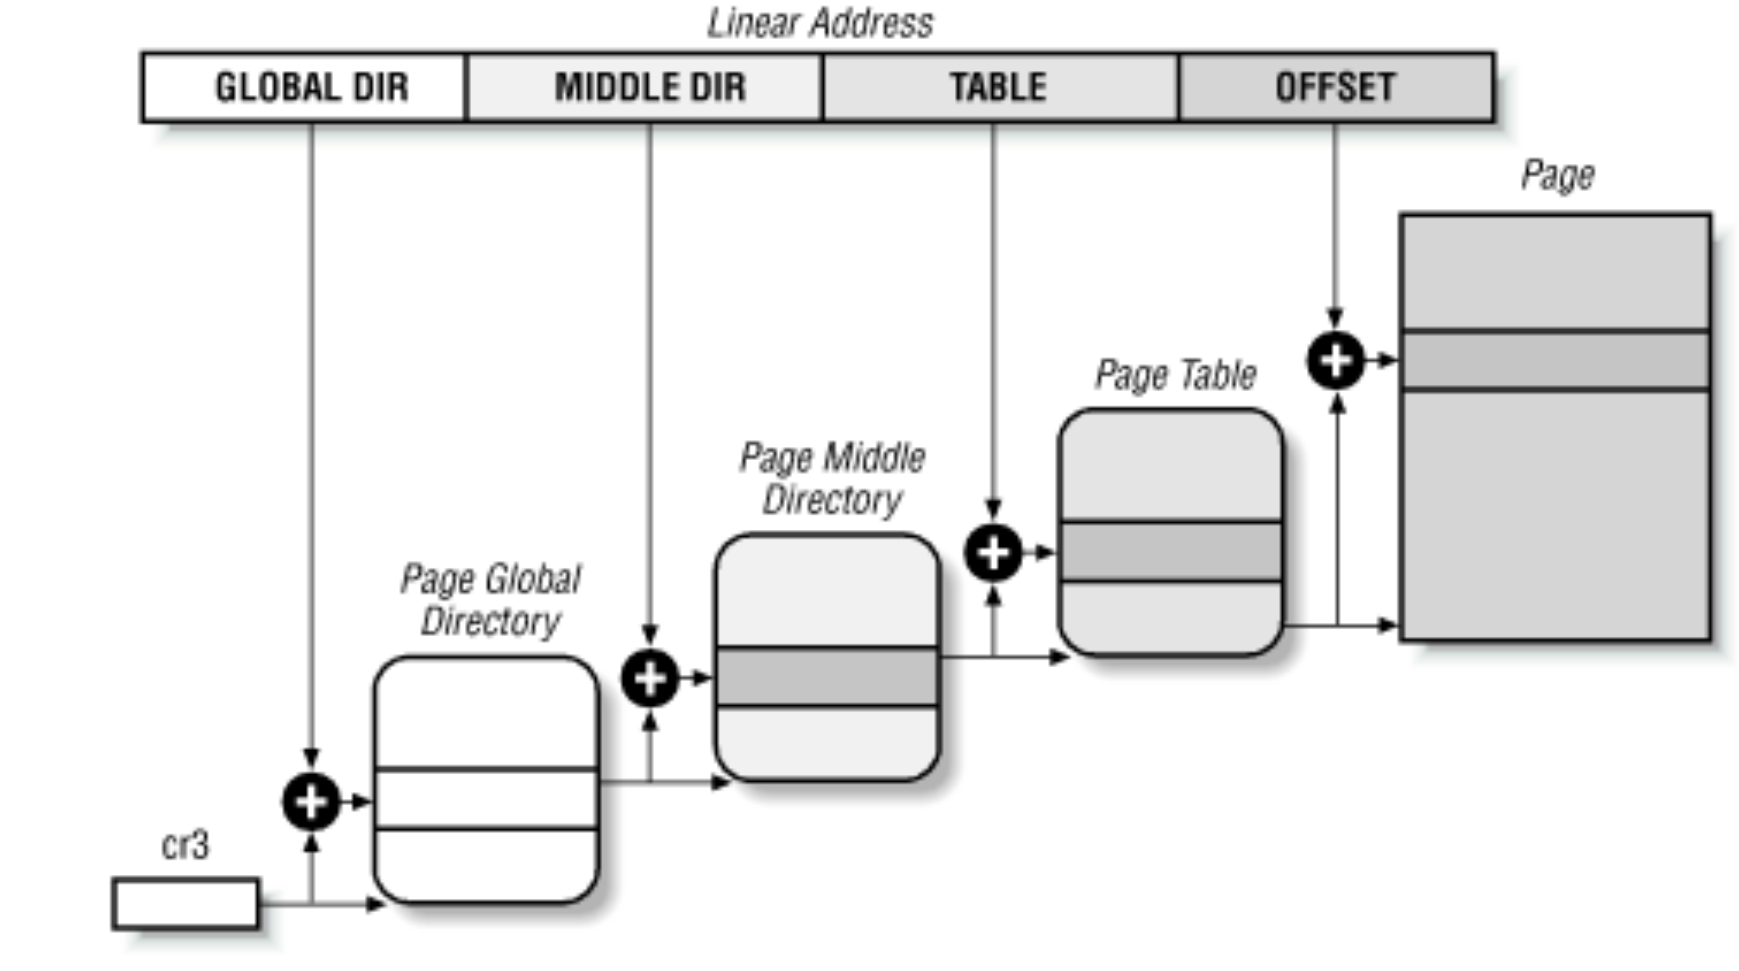
\includegraphics[width=0.8\textwidth]{linuxvm.png}
  \fig{1}{0 pt}{Linux Page Tables ($<$ v.2.10)}
\end{center}

Linux adopts a common paging model that fits both 32-bit and 64-bit architectures consisting of three-level paging up to kernel v.2.10 and four-level paging from kernel 2.11 introducing the Page Upper Directory as second level before Page Middle Directory (refer to Figure 5.1). Such scheme allows the kernel to be highly architecture independent reducing the amount of code needed to write for specific architectures. Various macros are then used to map the paging scheme that Linux uses to the
hardware specific paging scheme. \marginnote{\texttt{x_SIZE =} $2^{\texttt{x_SHIFT}}$ \\ Also \texttt{PTRS_PER_x} are defined to determine the number of entries in each level of the page table}[5cm]


\begin{center}
  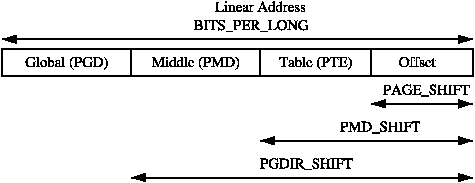
\includegraphics[width=0.75\textwidth]{bits1.png}
\end{center}


\begin{center}
  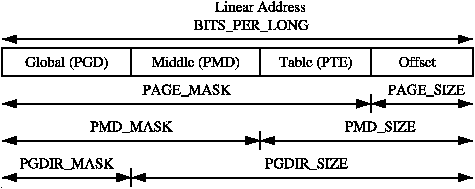
\includegraphics[width=0.75\textwidth]{bits2.png}
  \fig{2}{0 pt}{Macros for paging mapping}
\end{center}

All the page tables entry types are defined through structs like \texttt{typedef struct \{unsigned long pte_low; \} pte_t} to ensure typechecking when manipulating table entries.

Various masks are defined in order to perform easy checks on page table entries such as \texttt{_PAGE_PRESENT} to be used as follows:

\begin{verbatim}
    pte_t x;

    x = ...;

    if ((x.pte_low) & _PAGE_PRESENT) {
        /* executed if true */
    }
\end{verbatim}

Also multiple types of page entry flags are defined for the most common types of combinations of them such as \texttt{PAGE_SHARED, PAGE_KERNEL, PAGE_READONLY} etc.


\section{Kernel Page Table Initialization}

When carrying out the setup of architecture specific data structures in \texttt{setup_arch()}, also the transition from 8MB to 896MB is performed in \texttt{paging_init()} found in \\ \texttt{arch/i386/mm/init.c} of which main subroutine is the following.

\begin{verbatim}
> arch/i386/mm/init.c
    static void __init pagetable_init (void) {
        end = (unsigned long)__va(max_low_pfn*PAGE_SIZE);

        pgd_base = swapper_pg_dir;
        i = __pgd_offset(PAGE_OFFSET);
        pgd = pgd_base + i;

        for (; i < PTRS_PER_PGD; pgd++, i++) {
            vaddr = i*PGDIR_SIZE;
            if (end && (vaddr >= end)) break;
            pmd = (pmd_t *)pgd;
            ... 
            for (j = 0; j < PTRS_PER_PMD; pmd++, j++) {
                vaddr = i*PGDIR_SIZE + j*PMD_SIZE;
                if (end && (vaddr >= end))
                    break;
                ...
                pte_base = pte = (pte_t *) alloc_bootmem_low_pages(PAGE_SIZE);
                for (k = 0; k < PTRS_PER_PTE; pte++, k++) {
                    vaddr = i*PGDIR_SIZE + j*PMD_SIZE + k*PAGE_SIZE;
                    if (end && (vaddr >= end)) break;
                    *pte = mk_pte_phys(__pa(vaddr), PAGE_KERNEL);
                }
                set_pmd(pmd, __pmd(_KERNPG_TABLE + __pa(pte_base)));
                ...
            }
        }... }
\end{verbatim}

In the snippet shown above \texttt{end} is \texttt{0xf8000000} (128 MB short 4GB) and \texttt{i} is \texttt{0xc0000000} meaning that those are the virtual addresses used by the kernel. The routine uses the bootmem alocator to allocate Page Tables (last level) therefore the page tables might not be stored contiguously in memory. The function maps linearly the virtual addresses \texttt{0xc0000000} to \texttt{0xf8000000} to the first 896MB of page frames of physical memory.

Once the paging is setup we must ensure that no old entry is cached in the
TLB. This is done in \texttt{paging_init()} by calling 
\texttt{load_cr3(swapper_pg_dir)} and \texttt{__flush_tlb_all()}.

\begin{verbatim}
> include/asm-i386/processor.h
    #define load_cr3(pgdir) \
        asm volatile( "movl %0, %%cr3": : "r" (__pa(pgdir)) );
\end{verbatim}

As shown above, in \texttt{\%cr3} is written \texttt{swapper_pg_dir}.
This is done because the page tables used up to now might not be the ones
in \texttt{swapper_pg_dir} (following the execution path from
\texttt{arch/i386/kernel/head.S}) but the ones setup by the boot process
which might have launched the kernel from a different entry point.
Most of the \texttt{i386} architectures ensure that
the TLB is flushed if the \texttt{\%cr3} register is written but
there can still be some architectures that need further instructions to ensure that
the TLB is indeed flushed and in that case this is done through
\texttt{__flush_tlb_all()}.

In newer versions of the kernel (v. 4.16) \texttt{load_cr3()} is
reimplemented as follws:

\begin{verbatim}
> arch/x86/include/asm/special_insns.h 
    ...
    static inline void native_write_cr3(unsigned long val) {
        asm volatile( "movl %0, %%cr3": : "r" (val), "m" (__force_order)) );
    }
    ...
    static inline void load_cr3(pgd_t *pgdir) {
        native_write_cr3(__pa(pgdir));
    }   
\end{verbatim}

The motive of \texttt{__force_order} is nicely explained in a comment within
the file in which the functions are implemented.

\begin{verbatim}
> arch/x86/include/asm/special_insns.h 
/*
 * Volatile isn't enough to prevent the compiler from reordering the
 * read/write functions for the control registers and messing everything up.
 * A memory clobber would solve the problem, but would prevent reordering of
 * all loads stores around it, which can hurt performance. Solution is to
 * use a variable and mimic reads and writes to it to enforce serialization
 */
\end{verbatim}

\subsection{TLB APIs}
\label{subsec:TLB APIs}

The types of TLB events can be classified across two main characteristics:
scale and typology. When some event affects virtual addresses accessible
by every CPU/core in real-time-concurrency its scale is said to be
\textit{global}, instead if it affects only virtual addresses accessible
in time-sharing concurreny it is said to be \textit{local}.
The typology classification of events describes whether it is a virtual
to physical address remapping or virtual address access rule modification.

Other considerations needed to be done when dealing with TLB flushing is
its costs in terms of performance. Costs can be split into two sets: direct
costs and indirect costs. The former are the latency of the firmware to
perform the invalidation of the entries in the TLB plus the cost for
cross-CPU coordination. The latter is about the costs of TLB renewal
latency by the MMU firmware upon misses in the translation process.

The linux kernel provides various APIs for dealing with flushes of the
TLB that are then mapped to architecture dependent instructions. While
the APIs provide the possibility to perform selective flushing\footnote{
flushing just a subset of the entries in the TLB.}, the real effect
that it will have on the TLB depends on the instructions provided by the
firmware. Nevertheless it is highly recommended to use the most specific
API which is effective for the task and that doesn't make the software
too complex. Follow the interfaces provided by the linux kernel nicely
described under \texttt{Documentation/cachetlb.txt}.

\begin{description}
    \itemsep0pt
    \item \texttt{flush_tlb_all(void)} Flushes the entire TLB on
        \textit{all} processors running in the system and it is usually
        invoked when the kernel page tables change since they are global
        by nature. Its implementation is based on a function that allows
        to execute a portion of code on all processors based on IPIs.
        Such portion of code is \texttt{__flush_tlb_all}.
    \item \texttt{flush_tlb_mm(struct mm_struct *mm)} Flushes all the TLB
        entries related to a user address space. This is invoked usually
        when it is needed to invalidate all entries associated to a process
        for example when performing a \texttt{fork()} to make the address
        space not writable for COW (Copy on Write). On some architectures
        (MIPS) this is required for all cores instead of affecting only
        the local processor.
    \item \texttt{flush_tlb_range(struct mm_struct *mm, unsigned long
        start, \\ unsigned long end)} Similarly to the function above it is
        used to flush a range of (user) virtual addresses translations from
        the TLB. Primarily, this is used for \texttt{munmap()/mremap()} or
        \texttt{mprotect()}. The interface is provided in hopes that the
        port can find a suitably efficient method for removing multiple page
        sized translations from the TLB instead of having the kernel call
        \texttt{flush_tlb_page} for each entry which may be modified.
    \item \texttt{flush_tlb_page(struct vm_area_struct *vma, unsigned long
        page)} Flushes a single page from the TLB. Mainly used for flushing
        the TLB entry of some page after it has been paged out or faulted in
        meaning that the access to that page caused a fault (for example COW).
    \item \texttt{flush_tlb_pgtables(struct mm_struct *mm, unsigned long
        start, \\ unsigned long end)} Used when page tables of some software
        are being torn down. Some platforms cache the lowest level of the
        page tables in a linear virtually mapped array, to make TLB miss
        processing more efficient. In these cases the TLB needs to be flushed
        when parts of the page tables tree are unlinked/freed.
    \item \texttt{update_mmu_cache(struct vm_area_struct *vma, unsigned long
        address, \\ pte_t pte)} Used to inform the CPU that there exists
        a translation for the virtual address \texttt{address} corresponding
        to the entry \texttt{pte}. Such information can be used in many ways
        by the CPU such as deciding whether to flush its data cache or
        preload TLB translations.
\end{description}

\section{NUMA}

\begin{center}
  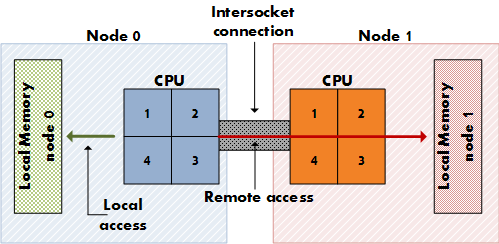
\includegraphics[width=0.6\textwidth]{numa.png}
  \fig{3}{0 pt}{NUMA systems}
\end{center}

With the ever growing disparity between the performance of processors and
memory, memory accesses started to became a bottleneck in multi processor
systems. This issue is addressed by arranging memory into banks and assigning
each bank to one or a set of cores. We denote by the term \textit{node} the
set of cpus and banks coupled together. All cores can access all the memory but
depending on their distance from the banks the cost to access memory is
different. Such architectures are defined as Non-Uniform Memory Access
(NUMA).

\newpage
\bibliography{Lec5}
\bibliographystyle{plainnat}
\end{document}
